\documentclass{article}

\usepackage[utf8]{inputenc} %Only required if not using XeLatex
\usepackage[T1]{fontenc}
\usepackage[final]{microtype}
\usepackage{bm} %Bold font for math equations

\usepackage{helvet} %Set font type (helvetica)
\renewcommand{\familydefault}{phv} %Set helvetica as default font

\usepackage[a4paper]{geometry} %Setting document size and margin width

\usepackage{enumitem} %Custom list
\newlist{arrowlist}{itemize}{1} %Define custom list name
\setlist[arrowlist]{label=$\Rightarrow$} %Define arrow for custom list label

\usepackage{graphicx} %Required for graphics and figures
\graphicspath{ {./Fig/} }
\usepackage[export]{adjustbox} %Used for adjusting image box
\usepackage{caption} %For caption customizations
\usepackage{subcaption}
\usepackage{float} %For [H] options of inserting figure

\usepackage{hyperref} %For url

\title{\textbf{Uncertainty Quantification of Plasma Filament in the Tokamak Scrape-off Layer}}
\author{Jasper Ng}
\date{May 2025}

\begin{document}

\maketitle

\noindent{\textbf{\Large Project Log}}

\begin{arrowlist}
    \item \textbf{Week starting from 02/04/2025}
    \begin{itemize}
        \item Discussed about the project specifics:
        \begin{itemize}
        	\item Premise of the project
        	\item Computational and physics aspects
            \begin{itemize}
        		\item[] Computational:
                \begin{itemize}
        			\item Use of Linux to compile C/C++ programmes
        			\item Use of Blob2d from BOUT++ framework
        			\item Use python for "gluing" everything together
                \end{itemize}
        		\item[] Physics:
                \begin{itemize}
        			\item Plasma filament occur in SOL of MCF fusion plasmas
        			\item Filaments created due to ExB forces
        			\item Blob size with different motions
                \end{itemize}
            \end{itemize}
        	\item Goals and objectives
        \end{itemize}
        \item Reading materials related to project
        \begin{itemize}
        	\item Plasma filament
        	\item Application of Gaussian process on tearing modes
        \end{itemize}
    \end{itemize}
    
    \item \textbf{Week starting from 04/03/2025}
    \begin{itemize}
        \item Discussion on Gaussian processes and specifics on components and methods:
        \begin{itemize}
        	\item Covariance matrix of multivariate Gaussian functions
        	\item Kernels for Gaussian processes
        \end{itemize}
        \item Risk assessment reviewed and submitted
    \end{itemize}
    
    \item \textbf{Week starting from 14/03/2025}
    \begin{itemize}
        \item Discussion on project specifics
        \begin{itemize}
        	\item Computational: Focus on environmental variables not numerical variables
        	\item Application of Gaussian process on plasma filament (blobs)
        \end{itemize}
        \item Version control training
    \end{itemize}
    
    \item \textbf{Week from 27/03/2025}
    \begin{itemize}
        \item Project objectives for the coming weeks
        \begin{itemize}
        	\item Install gcc on WSL
        	\item Compile BOUT++ and build programme
        	  \item Blob2d compiled and performed test runs
        	\item Create local and GitHub repository	
        	\item Create project log
        \end{itemize}
        \item Lay summary and Literature review
        \begin{itemize}
        	\item Deadline 08/05/2025
        	\item  Record literature in Zotero
        \end{itemize}
    \end{itemize}
    
    \item \textbf{Week from 15/04/2025}
    \begin{itemize}
        \item Discussion on coding specifics, and flags for compiling BOUT++ as well as running blob2d
        \begin{itemize}
            \item Record method of compilation such as use of cmake, and any flags/checks used
            \item Generally, less checks = faster runs, and checks include (refer to bout-dev build guide for checks):
            \begin{itemize}
                \item DCMAKE\_CXX\_FLAGS="-03"
                \item DBUILD\_TYPE=Debug
                \item DCHECK=0
            \end{itemize}
            \item Documentation for bout-dev: \url{https://bout-dev.readthedocs.io/en/latest/user_docs/quickstart.html#running-bout}
            \item Documentation for xbout module: \url{https://xbout.readthedocs.io/en/latest/index.html}, used for analysing results from BOUT++ runs
            \item For applying more cores for application run, use command "mpirun -n x" with x for amount of cores
            \item Github repository created to track project progress: \url{https://github.com/wxj512/Dissertation-Project.git}
        \end{itemize}
    \end{itemize}
    
    \begin{figure}[H]
    \centering
        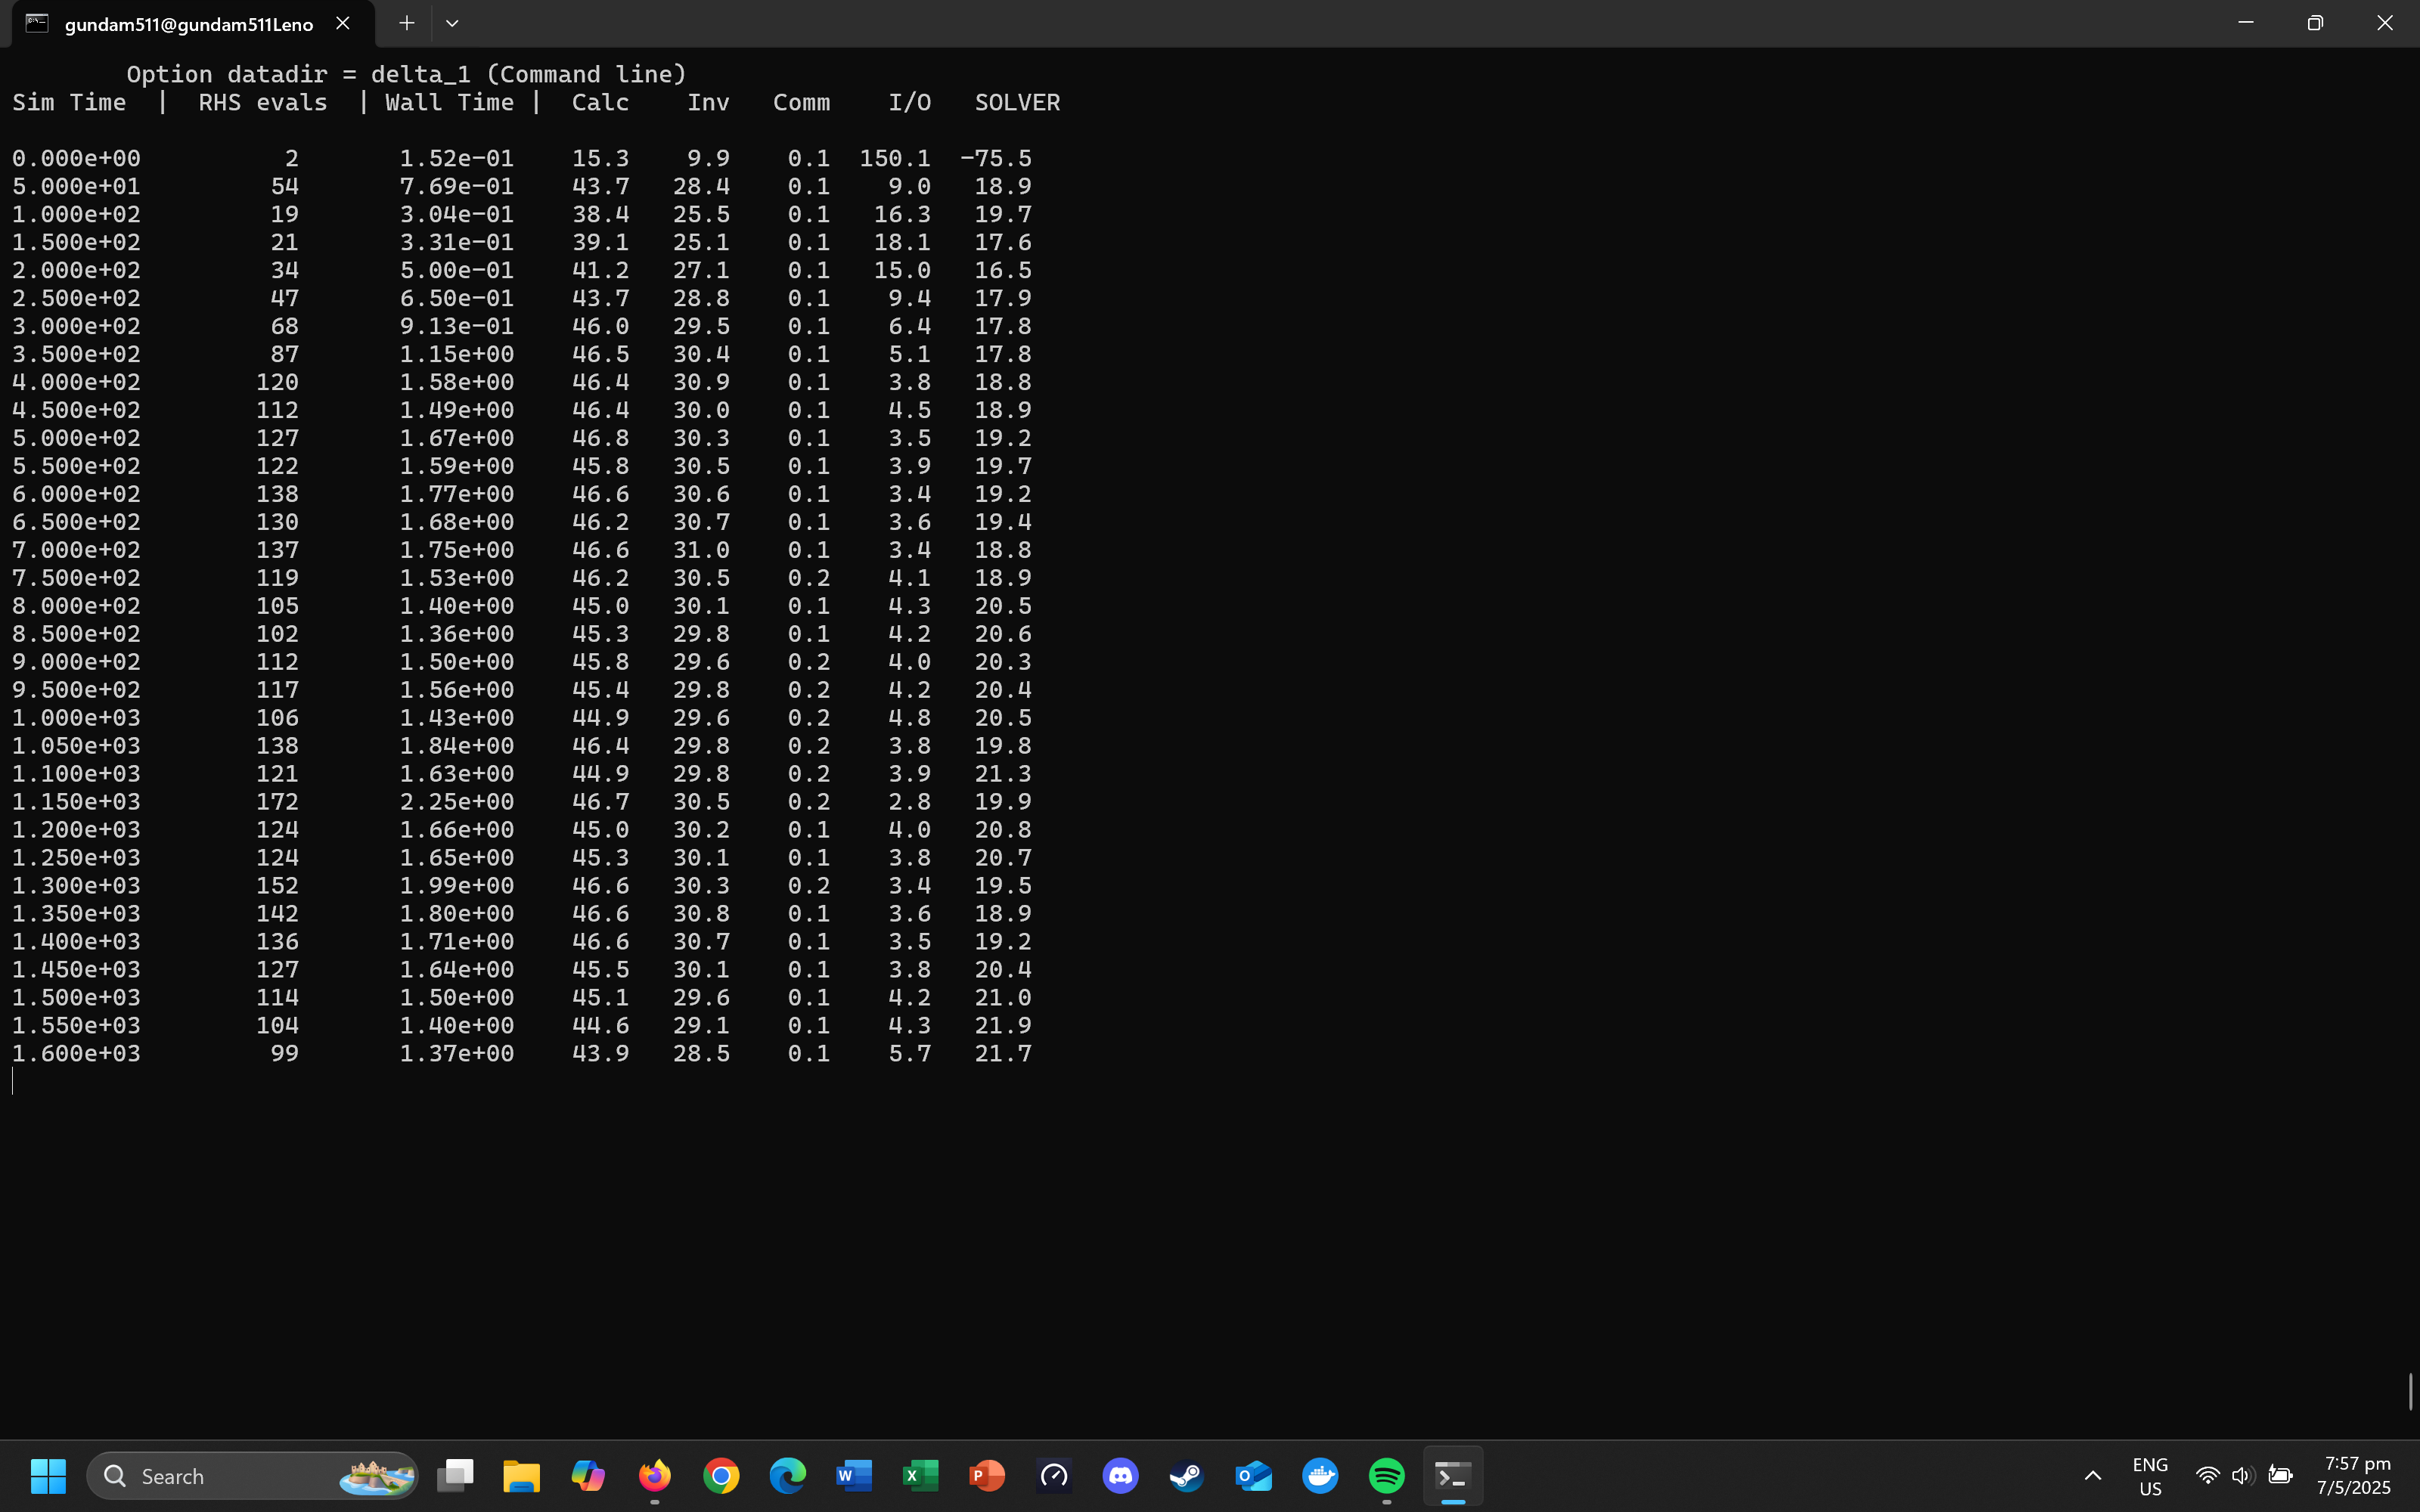
\includegraphics[height=0.3\textheight]{./Fig/Fig1 blob2d example run.png}
        \normalsize{\caption{Console view of blob2d run}}
        \label{fig:fig1}
    \end{figure}   

    \begin{figure}[H]
    \centering
        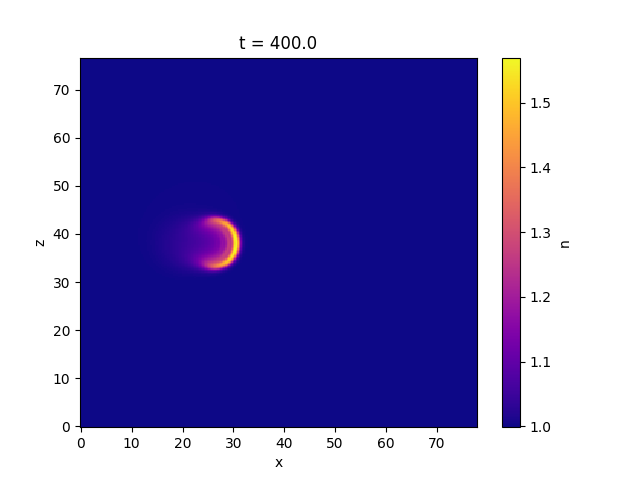
\includegraphics[height=0.5\textheight]{./Fig/Fig2 blob at t 400.png}
        \normalsize{\caption{Density (n) of blob at t=400s using input conditions from delta\_1 example}}
        \label{fig:fig2}
    \end{figure}   
    
    
    \item \textbf{Week from 29/04/2025}
       \begin{itemize}
            \item Drafted and finished literature review
            \item Refer to Lit\_rev\_plan.tex for details (could be found on Github repository)
       \end{itemize}
\end{arrowlist}

\end{document}